\documentclass[a4paper,11pt]{jarticle}

% レイアウト
\setlength{\hoffset}{0cm}
\setlength{\oddsidemargin}{-3mm}
\setlength{\evensidemargin}{-3cm}
\setlength{\marginparsep}{0cm}
\setlength{\marginparwidth}{0cm}
\setlength{\textheight}{24.7cm}
\setlength{\textwidth}{17cm}
\setlength{\topmargin}{-45pt}


\renewcommand{\baselinestretch}{1.2}
\renewcommand{\floatpagefraction}{1}
\renewcommand{\topfraction}{1}
\renewcommand{\bottomfraction}{1}
\renewcommand{\textfraction}{0}
\renewcommand\thefootnote{\arabic{footnote})}

% パッケージ
\usepackage[dvipdfmx]{graphicx}
\usepackage{amsmath,amssymb,epsfig}
\usepackage{eucal}
\usepackage{bm}
\usepackage{ascmac}
\usepackage{pifont}
\usepackage{multirow}
\usepackage{enumerate}
\usepackage{cases}
\usepackage{type1cm}
\usepackage{cancel}
\usepackage{url}
\usepackage{cite}
%\usepackage{color}
\usepackage[dvipdfmx]{color}
\usepackage{caption}
\usepackage[caption=false]{subfig}
\captionsetup[figure]{labelsep=space}
\usepackage{here}

% 擬似コード作成用
\usepackage[ruled,vlined]{algorithm2e}
\usepackage{setspace}
\DeclareRelationFont{JY1}{mc}{it}{}{OT1}{cmr}{it}{}
\DeclareRelationFont{JT1}{mc}{it}{}{OT1}{cmr}{it}{}
\DeclareFontShape{JY1}{mc}{m}{it}{<5> <6> <7> <8> <9> <10> sgen*min
    <10.95><12><14.4><17.28><20.74><24.88> min10
    <-> min10}{}
\DeclareFontShape{JT1}{mc}{m}{it}{<5> <6> <7> <8> <9> <10> sgen*tmin
    <10.95><12><14.4><17.28><20.74><24.88> tmin10
    <-> tmin10}{}
\DeclareRelationFont{JY1}{mc}{sl}{}{OT1}{cmr}{sl}{}
\DeclareRelationFont{JT1}{mc}{sl}{}{OT1}{cmr}{sl}{}
\DeclareFontShape{JY1}{mc}{m}{sl}{<5> <6> <7> <8> <9> <10> sgen*min
    <10.95><12><14.4><17.28><20.74><24.88> min10
    <-> min10}{}
\DeclareFontShape{JT1}{mc}{m}{sl}{<5> <6> <7> <8> <9> <10> sgen*tmin
    <10.95><12><14.4><17.28><20.74><24.88> tmin10
    <-> tmin10}{}
\DeclareRelationFont{JY1}{mc}{sc}{}{OT1}{cmr}{sc}{}
\DeclareRelationFont{JT1}{mc}{sc}{}{OT1}{cmr}{sc}{}
\DeclareFontShape{JY1}{mc}{m}{sc}{<5> <6> <7> <8> <9> <10> sgen*min
    <10.95><12><14.4><17.28><20.74><24.88> min10
    <-> min10}{}
\DeclareFontShape{JT1}{mc}{m}{sc}{<5> <6> <7> <8> <9> <10> sgen*tmin
    <10.95><12><14.4><17.28><20.74><24.88> tmin10
    <-> tmin10}{}
\DeclareRelationFont{JY1}{gt}{it}{}{OT1}{cmbx}{it}{}
\DeclareRelationFont{JT1}{gt}{it}{}{OT1}{cmbx}{it}{}
\DeclareFontShape{JY1}{mc}{bx}{it}{<5> <6> <7> <8> <9> <10> sgen*goth
    <10.95><12><14.4><17.28><20.74><24.88> goth10
    <-> goth10}{}
\DeclareFontShape{JT1}{mc}{bx}{it}{<5> <6> <7> <8> <9> <10> sgen*tgoth
    <10.95><12><14.4><17.28><20.74><24.88> tgoth10
    <-> tgoth10}{}
\DeclareRelationFont{JY1}{gt}{sl}{}{OT1}{cmbx}{sl}{}
\DeclareRelationFont{JT1}{gt}{sl}{}{OT1}{cmbx}{sl}{}
\DeclareFontShape{JY1}{mc}{bx}{sl}{<5> <6> <7> <8> <9> <10> sgen*goth
    <10.95><12><14.4><17.28><20.74><24.88> goth10
    <-> goth10}{}
\DeclareFontShape{JT1}{mc}{bx}{sl}{<5> <6> <7> <8> <9> <10> sgen*tgoth
    <10.95><12><14.4><17.28><20.74><24.88> tgoth10
    <-> tgoth10}{}
\DeclareRelationFont{JY1}{gt}{sc}{}{OT1}{cmbx}{sc}{}
\DeclareRelationFont{JT1}{gt}{sc}{}{OT1}{cmbx}{sc}{}
\DeclareFontShape{JY1}{mc}{bx}{sc}{<5> <6> <7> <8> <9> <10> sgen*goth
    <10.95><12><14.4><17.28><20.74><24.88> goth10
    <-> goth10}{}
\DeclareFontShape{JT1}{mc}{bx}{sc}{<5> <6> <7> <8> <9> <10> sgen*tgoth
    <10.95><12><14.4><17.28><20.74><24.88> tgoth10
    <-> tgoth10}{}
\DeclareRelationFont{JY1}{gt}{it}{}{OT1}{cmr}{it}{}
\DeclareRelationFont{JT1}{gt}{it}{}{OT1}{cmr}{it}{}
\DeclareFontShape{JY1}{gt}{m}{it}{<5> <6> <7> <8> <9> <10> sgen*goth
    <10.95><12><14.4><17.28><20.74><24.88> goth10
    <-> goth10}{}
\DeclareFontShape{JT1}{gt}{m}{it}{<5> <6> <7> <8> <9> <10> sgen*tgoth
    <10.95><12><14.4><17.28><20.74><24.88> tgoth10
    <-> tgoth10}{}
\endinput
%%%% end of jdummy.def

% カウンタの設定
\setcounter{section}{0}
\setcounter{subsection}{0}
\setcounter{subsubsection}{0}
\setcounter{equation}{0}

% キャプションの図をFigに変更
\renewcommand{\figurename}{Fig.}
\renewcommand{\tablename}{Tab.}

% 式番号を式(章番号.番号)に
\makeatletter
\renewcommand{\theequation}{\arabic{equation}}
\@addtoreset{equation}{section}
\makeatother

% タイトル部分
\title{\vspace{-20truemm}
{\normalsize \rightline{平成29年\ 7月\ 21日}}
{\large 制御系構成特論\\}
レポート課題1\\
\date{}
\vspace{-2truemm}}
\author{機械知能工学専攻 知能制御工学コース \hspace{3mm} 17344219 \ 二宮 悠二}
%---------------------------------------------
% ドキュメントの開始
\begin{document}
\parindent = 0pt % 字下げoff
% 表紙
\titlepage
\maketitle
%---------------------------------------------
% 課題内容
{\Large{\bf 問題}}
%---------------------------------------------
\begin{enumerate}
 \item {\bf Fig.}{\ref{blocks}}に示すブロック線図(a),(b)は等価である.このときの非構造的不確かさ$ \Delta a $を求めよ.
  \begin{figure}[H]
   \centering
   \subfloat[]{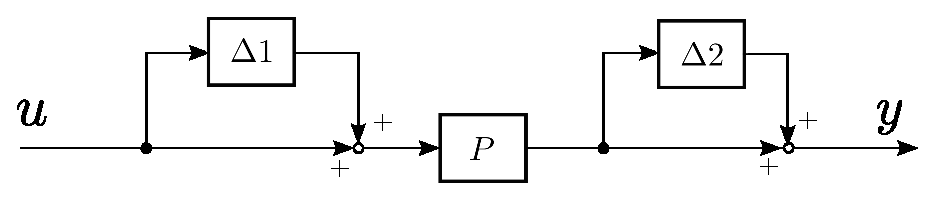
\includegraphics[scale=0.6]{../figure/eps/before.eps}}
  \\
   \vspace{0.5cm}
   \subfloat[]{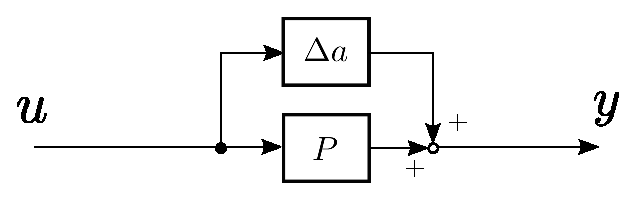
\includegraphics[scale=0.6]{../figure/eps/after.eps}}
  \\
   \caption{制御対象のブロック線図}
   \label{blocks}
  \end{figure}
 \item 次の式で与えられる関数の各ノルムを求めよ.\\
  \begin{equation}
   x(t) = \begin{cases} \nonumber
		 \begin{array}[t]{lc}
		  e^{-2t} & t \geq 0 \\
		  0       & t < 0 \\
		 \end{array}
		\end{cases}
  \end{equation}
\end{enumerate}
%---------------------------------------------
%---------------------------------------------
{\Large{\bf 解答}}
%---------------------------------------------
\begin{enumerate}
 \item 
\ \ {\bf Fig.}{\ref{blocks}} (a) の入出力関係は
\begin{equation}
 y = P(\Delta 1 + 1)(\Delta 2 + 1) u
\end{equation}
と表され,同図(b)は
\begin{equation}
 y = (P + \Delta a)u
\end{equation}
と表される.これら二式が等しくなるので,
\begin{equation}
 P(\Delta 1 + 1)(\Delta 2 + 1) u = (P + \Delta a)u
\end{equation}
が成り立つ.これを解くことにより
\begin{equation}
 \Delta a = P(\Delta 1 \Delta 2 + \Delta 1 + \Delta 2)
\end{equation}
を得る.
 \item 
\ \ $ {\cal L}_1 $ノルム,$ {\cal L}_2 $ノルム,$ {\cal L}_{\infty} $ノルムをそれぞれ$ \|x\|_1 $,$ \|x\|_2 $,$ \|x\|_{\infty} $とすると,各ノルムは次のように示される.
\begin{eqnarray}
 \|x\|_1 & = & \int_0^{\infty} e^{-2t} dt \nonumber \\
         & = & \left[- \dfrac{1}{2} e^{-2t} \right]^{\infty}_0 \nonumber \\
         & = & 0 + \dfrac{1}{2} \nonumber \\
         & = & \dfrac{1}{2} \\ \nonumber \\
 \|x\|_2 & = & \left( \int_0^{\infty} \left( e^{-2t} \right)^2 dt \right)^{\frac{1}{2}} \nonumber \\
         & = & \left( \left[ - {\dfrac{1}{4}}e^{-4t} \right]^{\infty}_0 \right)^{\frac{1}{2}} \nonumber \\
         & = & \left( {\dfrac{1}{4}} \right)^{\frac{1}{2}} \nonumber \\
         & = & \dfrac{1}{2} \\ \nonumber \\
 \|x\|_{\infty} & = & \sup_{t \geq 0} ~ e^{-2t} \nonumber \\
                & = & 1
\end{eqnarray}
\end{enumerate}




% % 図の挿入

% \begin{figure}[b]
%  \begin{center}
%   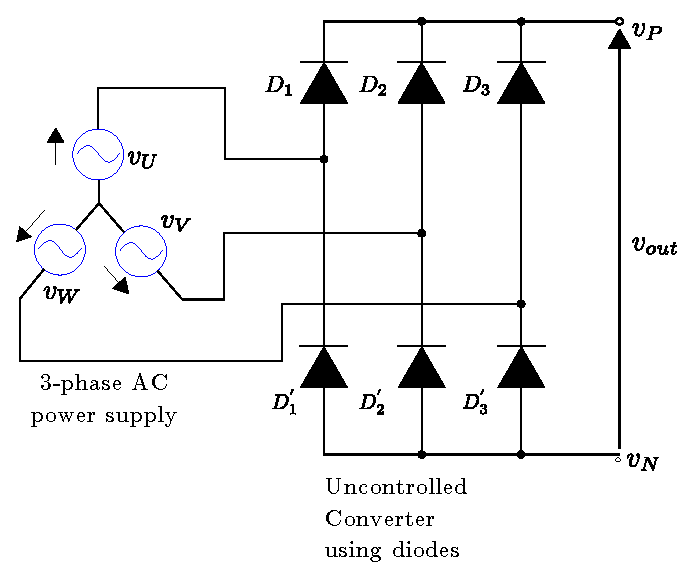
\includegraphics[scale=0.9]{../figure/circuit.eps}
%   \caption{Uncontrolled converter}
%   \label{circuit}
%  \end{center}
% \end{figure}


% % 表の挿入

% \begin{table}[htb]
%   \begin{center}
%     \caption{各素子のパラメータ}
%     \begin{tabular}{c|c|c} \hline
%       定数名[単位] & 記号 & 値 \\ \hline \hline
%       周波数[Hz] & $f_U,f_V,f_W$ & 120 \\ \hline
%                      & $\phi_U$ & $\frac{2\pi}{3}$ \\
%       初期位相角[rad] & $\phi_V$ & $\frac{4\pi}{3}$ \\
%                      & $\phi_W$ & $2\pi$ \\ \hline
%       抵抗[$\Omega$] & $R$ & 10 \\ \hline
%     \end{tabular}
%     \label{param}
%   \end{center}
% \end{table}


% % 図の挿入

% \begin{figure}[tb]
%  \centering
%  \vspace{0.5cm}
%  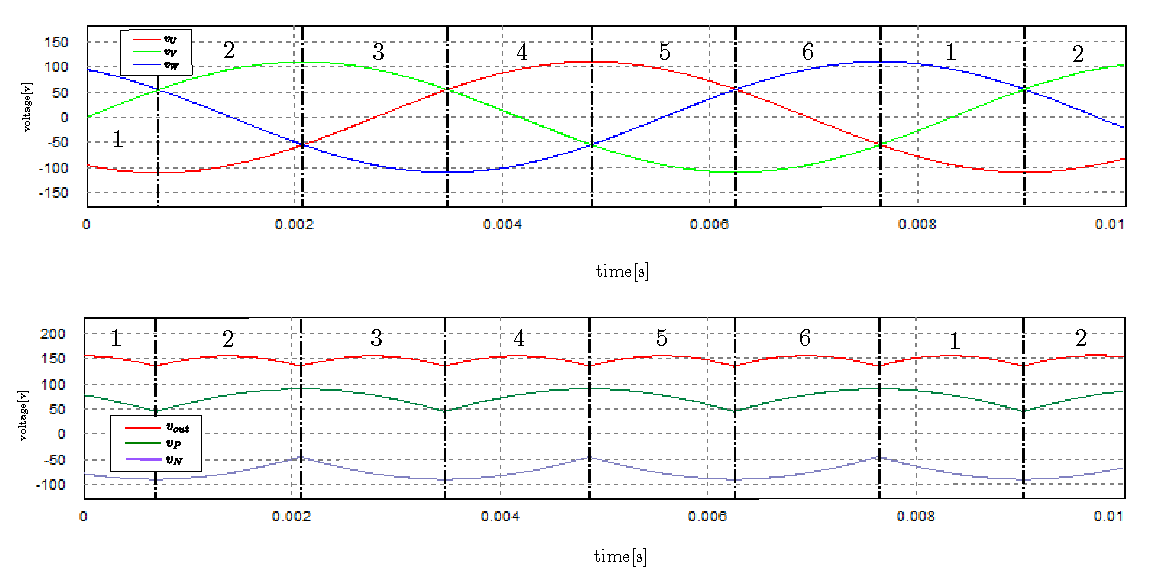
\includegraphics[scale=0.85]{../figure/waves.eps}\\
%  \hspace{0.0cm}
%  % 入力と出力\\
%  % \\
%  % \vspace{1.2cm}
%  % 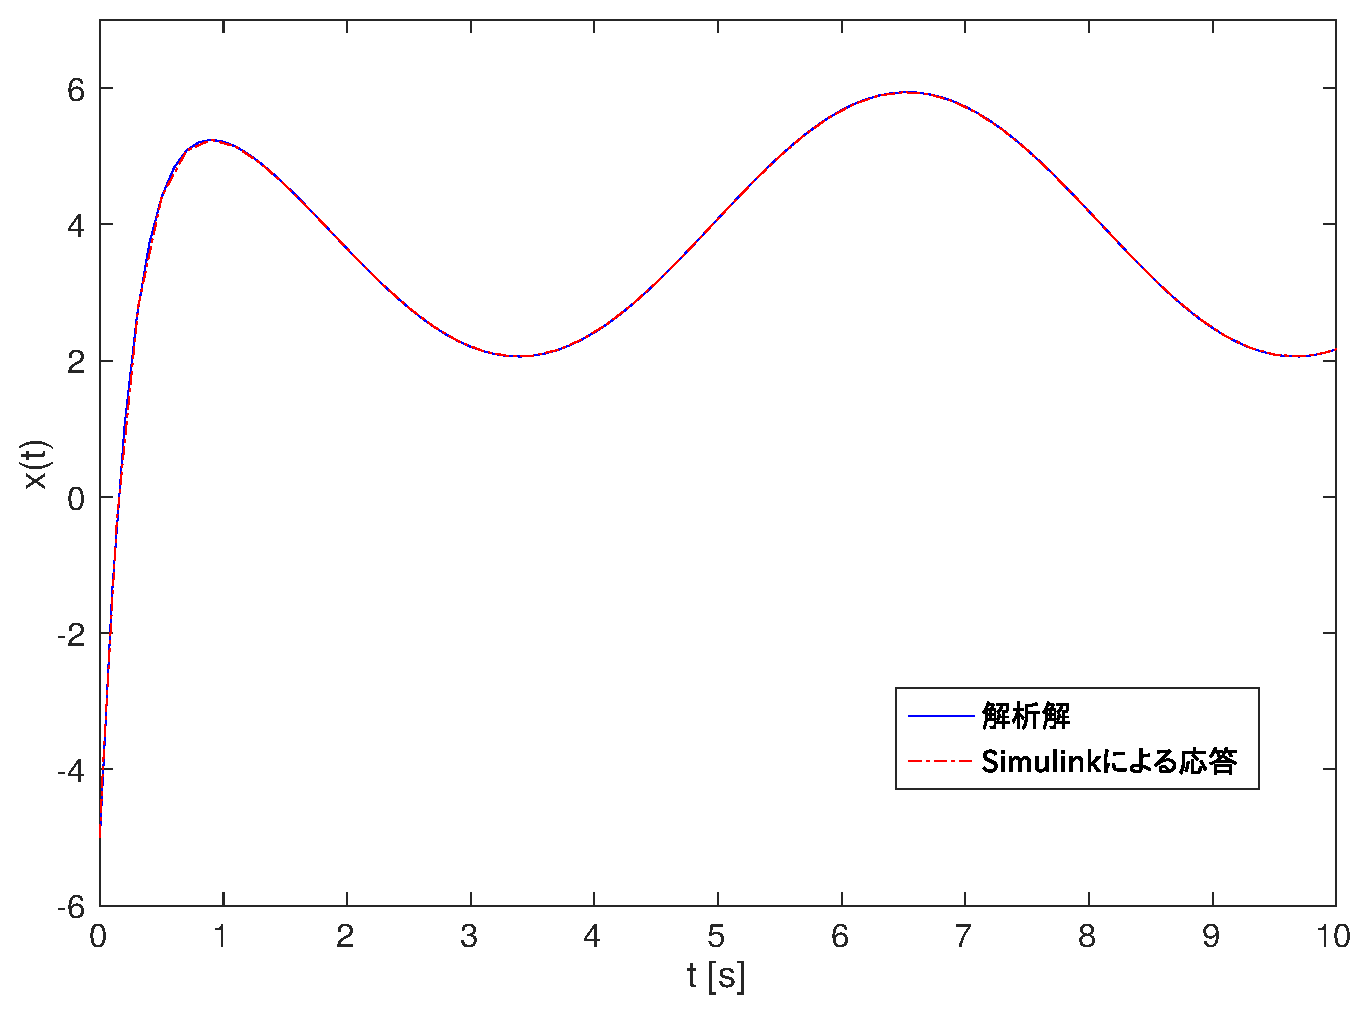
\includegraphics[scale=0.825]{../figure/output.eps}\\
%  % (b) 出力の電位\\
%  % \\
%  \caption{シミュレーションにより得られた各電源電圧(上)と出力電位(下)の波形}
%  \label{wave}
% \end{figure}

% \newpage

% % 図を並べて挿入

% \begin{figure}[tb]
%  \centering
%  \subfloat[区間1における回路動作]{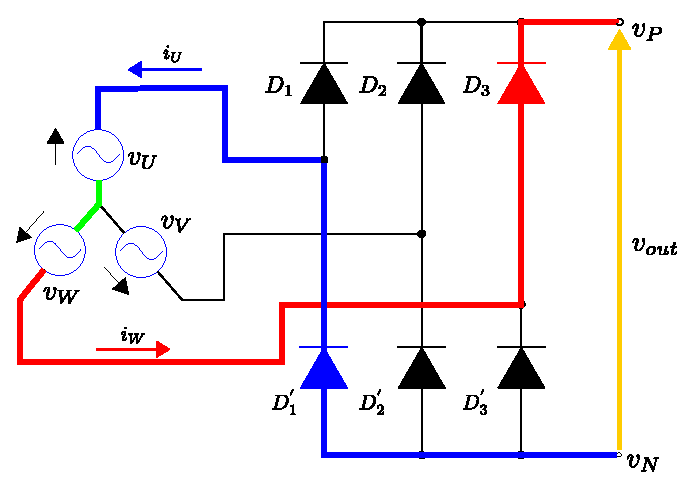
\includegraphics[scale=0.5]{../figure/kukan_1.eps}}
%  \hspace{1.5cm}
%  \subfloat[区間2における回路動作]{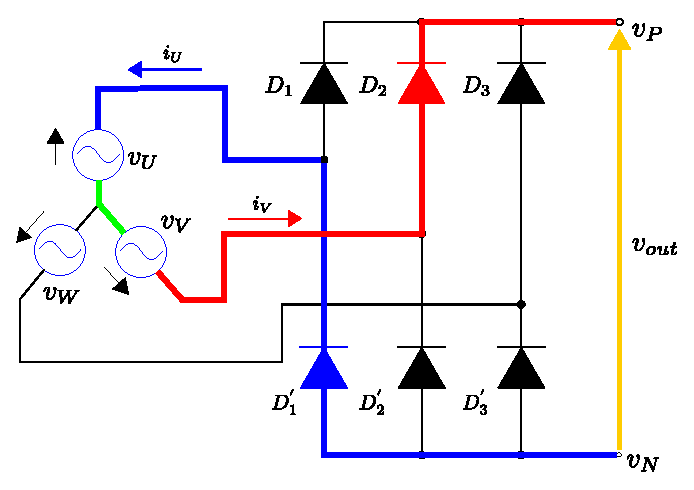
\includegraphics[scale=0.5]{../figure/kukan_2.eps}}
% \\
%  \vspace{0.5cm}
%  \subfloat[区間3における回路動作]{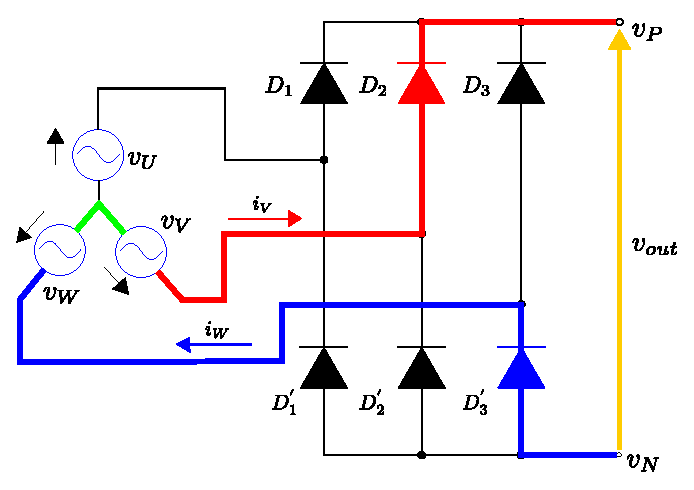
\includegraphics[scale=0.5]{../figure/kukan_3.eps}}
%  \hspace{1.5cm}
%  \subfloat[区間4における回路動作]{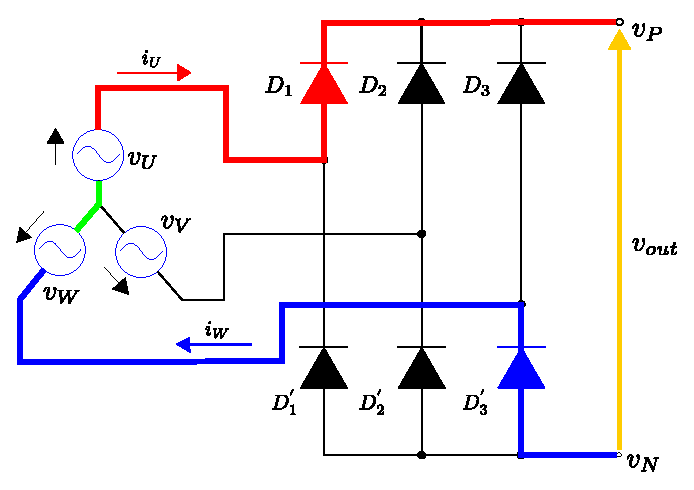
\includegraphics[scale=0.5]{../figure/kukan_4.eps}}
% \\
%  \vspace{0.5cm}
%  \subfloat[区間5における回路動作]{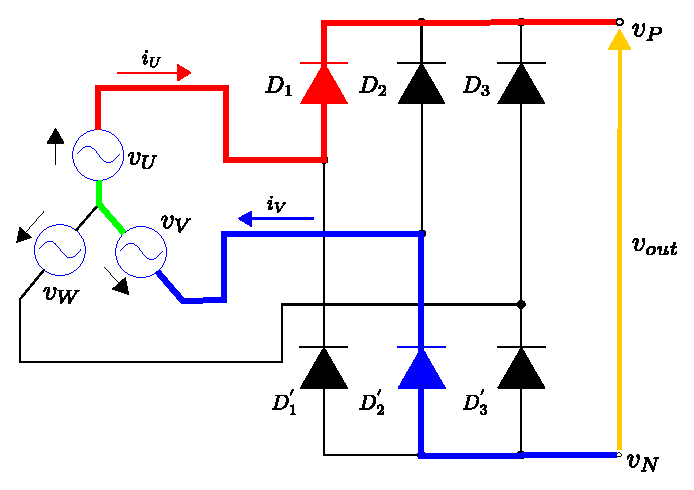
\includegraphics[scale=0.5]{../figure/kukan_5.eps}}
%  \hspace{1.5cm}
%  \subfloat[区間6における回路動作]{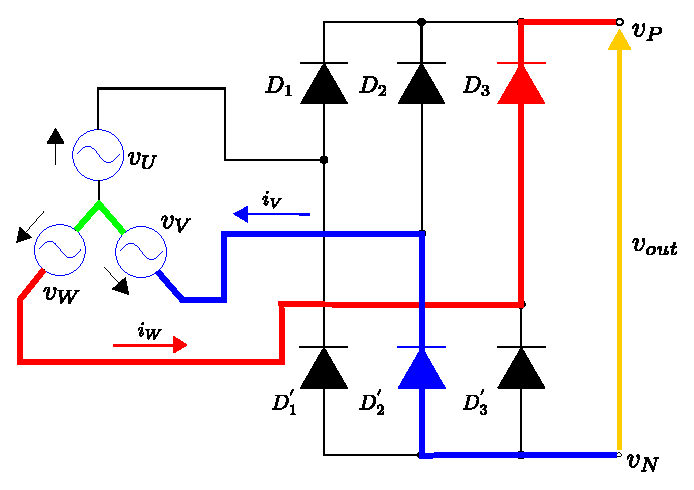
\includegraphics[scale=0.5]{../figure/kukan_6.eps}}
% \\
%  \caption{各区間での回路動作の様子}
%  \label{circuit_kaku}
% \end{figure}

% % 文中へのラベリング
% {\bf Fig. }\ref{circuit_kaku}に示す〜

% % 参考文献
% \begin{thebibliography}{99}
% \addcontentsline{toc}{section}{参考文献}
% \bibitem{1} T.Sakamoto,”Lecture Note of Advanced Electrical Drive Control System”,pp.19-20.
% \bibitem{2} 坪島 茂彦,”誘導電動機 -基礎から制御まで-”,東京電機大学出版局,pp.13-17,2006.
% \end{thebibliography}

\end{document}
